\section{Section: Prelude}

\section{Section Intro}

\begin{frame}[s]{This is the Plan}
  \small

  \begin{columns}[T]
    \begin{column}{.40\linewidth}
      \begin{enumerate}
        \item \textbf{Introducing Rosenpass}
        \item \textbf{The Design of Rosenpass}
        \item \textbf{Hybrid Security}
        \item \textbf{ChronoTrigger Attack}
        \item \textbf{Protocol Proofs} – big old rant!
      \end{enumerate}
    \end{column}
    \hfill
    \begin{column}{.55\linewidth}
      \centering
      \vspace{2.5em}
      This is an interactive talk. Ask questions during the talk. I would prefer this to turn into a conversation.
    \end{column}
  \end{columns}

	\vfill

    {
      \begin{tabular}[c]{@{\space}l}
      Follow the talk at:\\
      \footnotesize\href{github.com/rosenpass/slides/blob/main/2024-11-22-hpi/slides.pdf}{github.com/rosenpass/slides/blob/main/ 2024-11-22-hpi/slides.pdf}
      \end{tabular}
      \QRCode*{github.com/rosenpass/slides/blob/main/2024-11-22-hpi/slides.pdf}
    }

  \vfill

    \QRCode*{media.ccc.de/v/how-to-build-post-quantum-cryptographic-protocols-and-why-wall-clocks-are-not-to}\begin{tabular}[c]{@{\space}l}
    Rewatch at:\\
    \tiny\href{media.ccc.de/v/how-to-build-post-quantum-cryptographic-protocols-and-why-wall-clocks-are-not-to}{media.ccc.de/v/how-to-build-post-quantum-cryptographic-protocols-and-why-wall-clocks-are-not-to}
    \end{tabular}

  \vfill
\end{frame}



\begin{frame}{Introducing Rosenpass, briefly}
  \begin{columns}[fullwidth,c]

    \begin{column}{.7\linewidth}
      \begin{itemize}
        \item A post-quantum secure key exchange \textbf{protocol}
          {\small based on the paper Post-Quantum WireGuard~\citePqwg}
        \item An open source Rust \textbf{implementation} of that protocol, already in use
        \item A way to secure WireGuard VPN setups against quantum attacks
        \item A \textbf{post-quantum secure VPN}
        \item A governance \textbf{organization} to facilitate development, maintenance, and adoption of said protocol
        %\item A translation research organization
      \end{itemize}
      \bigskip
      \textbf{\url{rosenpass.eu}}
    \end{column}%
    \begin{column}{.3\linewidth}
      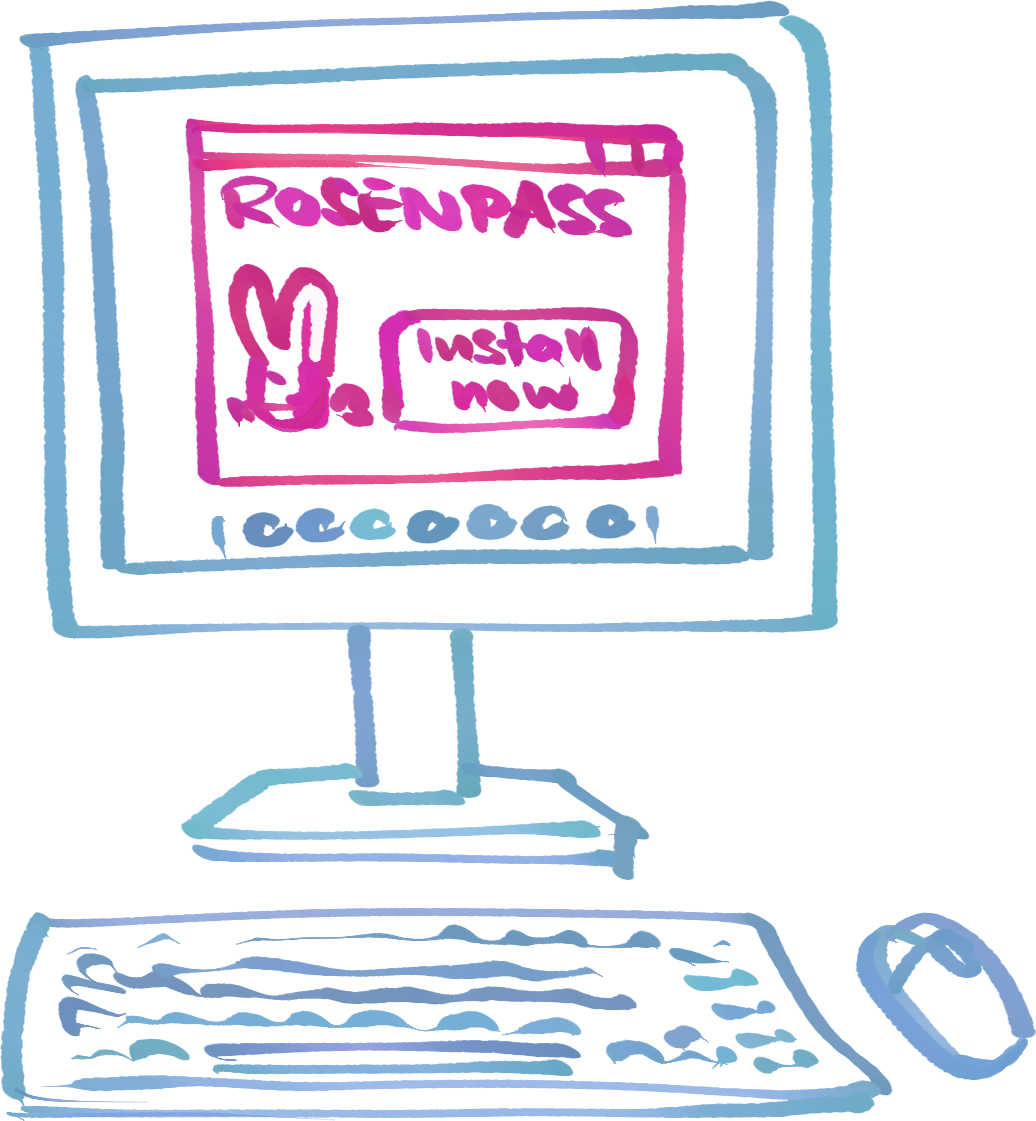
\includegraphics[ width=.92\linewidth]{graphics/Illu-install.png}
    \end{column}
  \end{columns}
\end{frame}
